% Provenance (never printed): cycle 3 / 6e "La planete Terre, l'environnement
% et l'action humaine" (the Earth in the Solar System; conditions for life);
% see sources/book1/PROVENANCE.md. Book 1, grade 6, chapter 1.
\chapter{The Earth, a Planet of the Solar System}\label{ch:g6:earth-a-planet}

Three robot probes have been sent out into space. One by one, they send
home a picture, like a postcard. The first comes from Venus: a pale ball
wrapped in thick \omterm{def:g4:clouds-rain-snow:cloud}{clouds}, where it is hot enough to melt lead and the air
presses on the ground with a crushing weight. The second comes from Mars:
a red, cold, dusty \omterm{def:g5:weather-and-climate:desert}{desert} under a thin sky. The third probe has turned its
camera back towards home: a blue and white ball, with \omterm{def:g2:water-on-earth:ocean}{oceans}, \omterm{def:g4:clouds-rain-snow:cloud}{clouds} and
ice. Three planets, neighbours around the same Sun. Why is only one of
them blue?
% ledger: nasa:venus-clouds, nasa:mars-water

\begin{omfigure}
\begin{minipage}[t]{0.31\linewidth}\centering
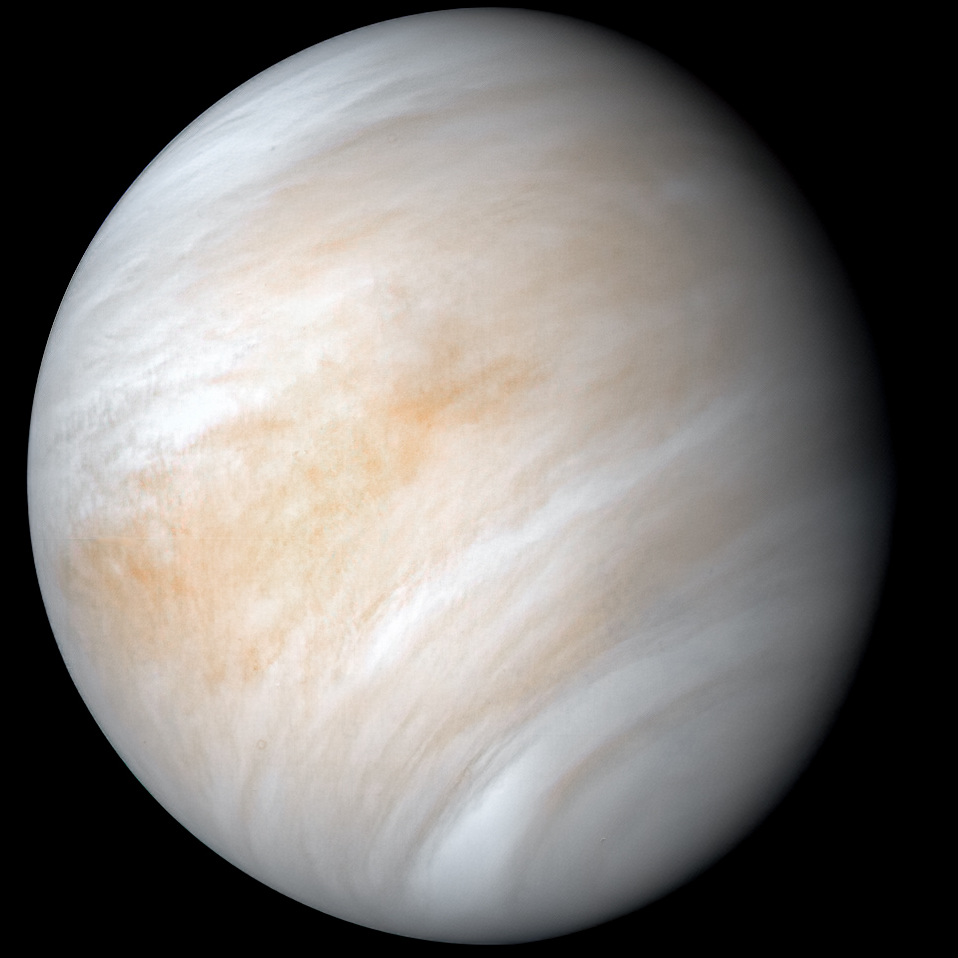
\includegraphics[width=\linewidth]{images/book1/g6-venus-mariner10.jpg}\\[2pt]
{\small Venus}
\end{minipage}\hfill
\begin{minipage}[t]{0.31\linewidth}\centering
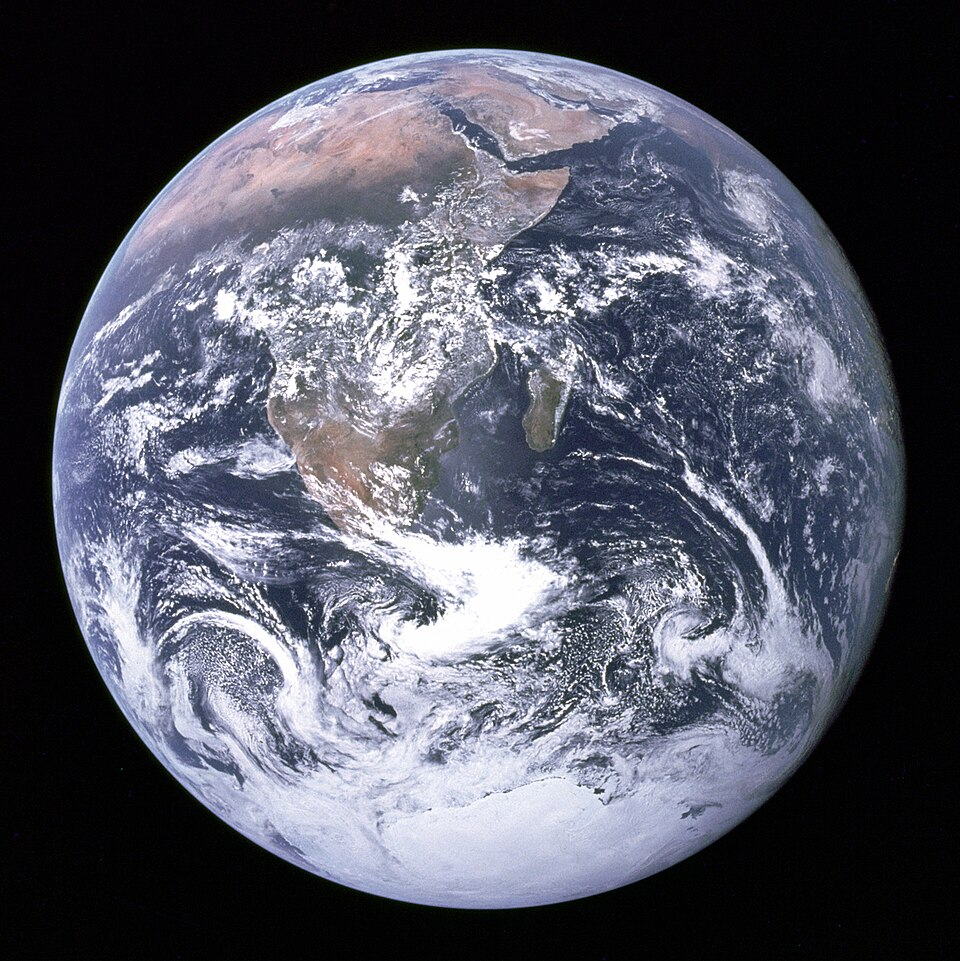
\includegraphics[width=\linewidth]{images/book1/g6-earth-apollo17.jpg}\\[2pt]
{\small The Earth}
\end{minipage}\hfill
\begin{minipage}[t]{0.31\linewidth}\centering
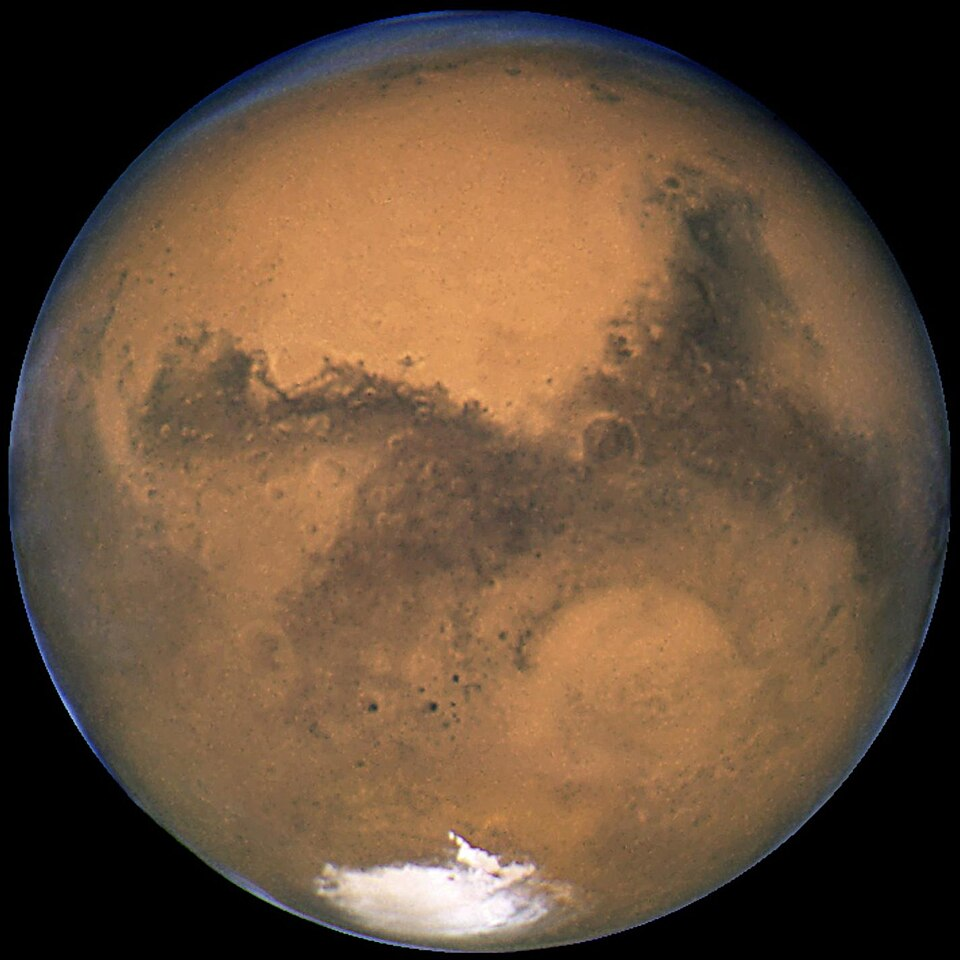
\includegraphics[width=\linewidth]{images/book1/g6-mars-hubble.jpg}\\[2pt]
{\small Mars}
\end{minipage}

\medskip
{\small Three postcards from space. Venus, photographed by the Mariner~10
probe in 1974: we see only the top of its \omterm{def:g4:clouds-rain-snow:cloud}{clouds}. The Earth, photographed
by the crew of Apollo~17 on their way to the Moon in 1972: Africa, Arabia
and the ice of Antarctica under white \omterm{def:g4:clouds-rain-snow:cloud}{clouds}. Mars, photographed by the
Hubble Space Telescope in 2003, with a white cap of ice at its \omterm{def:g3:continents-and-oceans:poles}{pole}.
(Photos: NASA/JPL-Caltech; NASA; NASA, ESA and the Hubble Heritage Team.)}
% ledger: nasa:venus-mariner10, nasa:apollo17-earth, hubble:mars-2003
\end{omfigure}

\begin{recall}
The physics books showed that the Sun is a star, a huge ball of hot gas
that shines by itself, and that a planet is a large round body that turns
around a star and does not shine by itself: we see it because it reflects
the light of its star. The Sun and everything that turns around it form
the Solar System. Each planet travels round the Sun along a path called
its orbit, and spins on itself around an axis. The air around us presses
on everything it touches: this is air pressure. The density of a material
tells how heavy a given volume of it is: one cubic centimetre of water
weighs 1~gram, so its density is 1~gram per cubic centimetre; a material
denser than water sinks in it, a material less dense floats. Finally, about seven tenths of
the Earth's surface is covered by the \omterm{def:g2:water-on-earth:ocean}{ocean}
(\cref{ch:g2:water-on-earth}).
\end{recall}

\section{Eight planets around the Sun}

Eight planets travel around the Sun. In order, from the closest to the
farthest, they are Mercury, Venus, the Earth, Mars, Jupiter, Saturn,
Uranus and Neptune. A sentence can help to remember the order: \emph{My
Very Easy Method Just Speeds Up Naming} (Mercury, Venus, Earth, Mars,
Jupiter, Saturn, Uranus, Neptune).

The drawing below shows the eight planets side by side, drawn to the same
scale: if a planet is twice as wide as another, its circle is twice as
wide too.

\begin{omfigure}
\pgfplotstableread{figdata/out/grade-6-planets-sizes.dat}\gsixsizes
\begin{tikzpicture}
  \draw[black!40] (-0.2,0) -- (13.8,0);
  \pgfplotstablegetrowsof{\gsixsizes}
  \pgfmathtruncatemacro{\gsixlast}{\pgfplotsretval-1}
  \foreach \i in {0,...,\gsixlast}{
    \pgfplotstablegetelem{\i}{x_cm}\of\gsixsizes \let\gx\pgfplotsretval
    \pgfplotstablegetelem{\i}{d_cm}\of\gsixsizes \let\gd\pgfplotsretval
    \pgfplotstablegetelem{\i}{name}\of\gsixsizes \let\gn\pgfplotsretval
    \pgfplotstablegetelem{\i}{d_km}\of\gsixsizes \let\gk\pgfplotsretval
    \pgfmathsetmacro{\gr}{\gd/2}
    \ifnum\i<4
      \fill[brown!70!black, draw=black!60, line width=0.3pt] (\gx,\gr) circle (\gr);
    \else
      \fill[orange!35, draw=black!60, line width=0.3pt] (\gx,\gr) circle (\gr);
    \fi
    \node[font=\scriptsize, rotate=40, anchor=north east, inner sep=1pt]
      at (\gx+0.08,-0.08) {\gn};
  }
  \node[font=\scriptsize, align=left, anchor=north west] at (-0.2,4.15)
    {\tikz\fill[brown!70!black, draw=black!60] (0,0) circle (2.2pt); rocky planets\\
     \tikz\fill[orange!35, draw=black!60] (0,0) circle (2.2pt); giant planets};
  \draw[|-|, black!70] (0,2.2) -- (1,2.2)
    node[midway, above, font=\scriptsize] {35\,000 km};
\end{tikzpicture}

{\small The eight planets drawn to scale (diameters from the NASA planetary
fact sheet). The distances between them are not to scale: they are far
too large to fit on any page.}
% ledger: planet:Mercury.diameter, planet:Venus.diameter, planet:Earth.diameter, planet:Mars.diameter, planet:Jupiter.diameter, planet:Saturn.diameter, planet:Uranus.diameter, planet:Neptune.diameter (figdata/grade-6/planets.py, part sizes)
\end{omfigure}

The four planets closest to the Sun are small. The next four are giants:
Jupiter is about 11 times as wide as the Earth. And the Sun? Drawn to the
same scale as the planets above, it would be a disc about 40~centimetres
across --- wider than this page.
% ledger: planet:Jupiter.diameter, planet:Earth.diameter, sun:R (planets.py: sun_cm = 39.9 cm)

Size is not the only difference. The table below gives, for each planet,
its diameter, its density (in grams per cubic centimetre), and its distance
from the Sun.

\begin{center}
\small
\begin{tabular}{lrrrr}
\hline
planet & diameter (km) & density (g/cm$^3$) & distance from the Sun (million km)\\
\hline
Mercury & 4\,879 & 5.4 & 58\\
Venus & 12\,104 & 5.2 & 108\\
Earth & 12\,756 & 5.5 & 150\\
Mars & 6\,792 & 3.9 & 228\\
\hline
Jupiter & 142\,984 & 1.3 & 779\\
Saturn & 120\,536 & 0.7 & 1\,432\\
Uranus & 51\,118 & 1.3 & 2\,867\\
Neptune & 49\,528 & 1.6 & 4\,515\\
\hline
\end{tabular}
% ledger: planet:Mercury.diameter, planet:Venus.diameter, planet:Earth.diameter, planet:Mars.diameter, planet:Jupiter.diameter, planet:Saturn.diameter, planet:Uranus.diameter, planet:Neptune.diameter, planet:Mercury.density, planet:Venus.density, planet:Earth.density, planet:Mars.density, planet:Jupiter.density, planet:Saturn.density, planet:Uranus.density, planet:Neptune.density, planet:Mercury.dist, planet:Venus.dist, planet:Earth.dist, planet:Mars.dist, planet:Jupiter.dist, planet:Saturn.dist, planet:Uranus.dist, planet:Neptune.dist (figdata/grade-6/planets.py, main table)
\end{center}

The densities split the planets into two families, with nothing in between:
the first four are dense, more than 3.9~grams per cubic centimetre, like
\omterm{def:g3:stones-pebbles-sand:rock}{rock} and metal; the last four are light, less than 1.7~grams per cubic
centimetre.

\begin{definition}[Rocky planets and giant planets]\label{def:g6:earth-a-planet:planet-types}
A \emph{rocky planet}\index{rocky planet} is a small, dense planet made of
\omterm{def:g3:stones-pebbles-sand:rock}{rock} and metal, with a solid surface on which a probe can land: Mercury,
Venus, the Earth and Mars. A \emph{giant planet}\index{giant planet} is a
very large planet of low density, made mostly of gases and liquids, with no
solid surface to land on: Jupiter, Saturn, Uranus and Neptune.
% ledger: nasa:planet-families
\end{definition}

\begin{omfigure}
\begin{minipage}[c]{0.6\linewidth}\centering
\begin{tikzpicture}
  \begin{axis}[ybar, bar width=11pt, width=\linewidth, height=5.4cm,
      ymin=0, ymax=6.2, xmin=-0.6, xmax=7.6,
      xtick={0,...,7}, xticklabels={Mercury,Venus,Earth,Mars,Jupiter,Saturn,Uranus,Neptune},
      xticklabel style={rotate=40, anchor=north east, font=\scriptsize},
      ytick={0,1,...,6}, ylabel={density (g/cm$^3$)},
      tick label style={font=\scriptsize}, label style={font=\scriptsize},
      axis x line*=bottom, axis y line*=left]
    \addplot[fill=brown!70!black, draw=black!60, bar shift=0pt, restrict x to domain=0:3]
      table[x=idx, y=density_gcm3] {figdata/out/grade-6-planets-density.dat};
    \addplot[fill=orange!35, draw=black!60, bar shift=0pt, restrict x to domain=4:7]
      table[x=idx, y=density_gcm3] {figdata/out/grade-6-planets-density.dat};
    \draw[blue!60!black, densely dashed] (axis cs:-0.6,1) -- (axis cs:7.6,1);
    \node[font=\scriptsize, blue!60!black, anchor=south, inner sep=1pt]
      at (axis cs:5,1) {water};
  \end{axis}
\end{tikzpicture}
\end{minipage}\hfill
\begin{minipage}[c]{0.36\linewidth}\centering
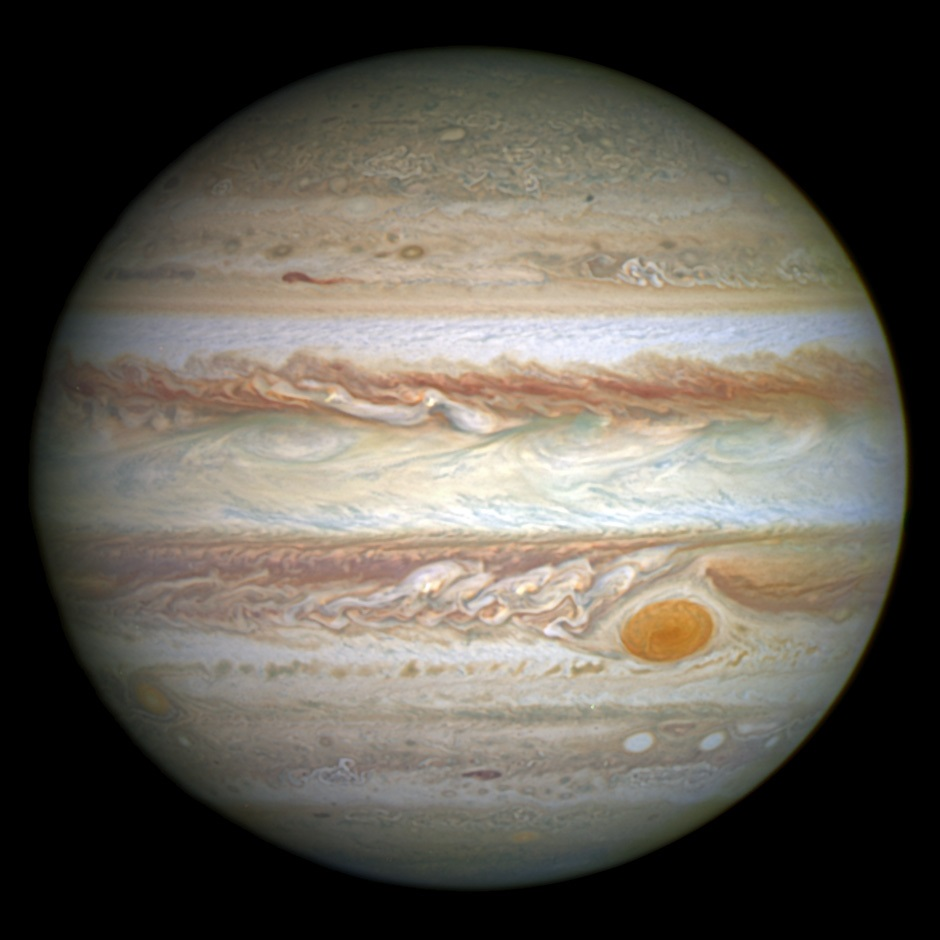
\includegraphics[width=0.9\linewidth]{images/book1/g6-jupiter-hubble.jpg}\\[2pt]
{\small Jupiter, photographed by the Hubble Space Telescope in 2014.
(Photo: NASA, ESA, A.~Simon.)}
% ledger: hubble:jupiter-2014
\end{minipage}

\smallskip
{\small Left: the density of the eight planets; the dashed line is the
density of water. Right: what we see of a \omterm{def:g6:earth-a-planet:planet-types}{giant planet} is the top of its
\omterm{def:g4:clouds-rain-snow:cloud}{clouds}.}
% ledger: planet:Mercury.density, planet:Venus.density, planet:Earth.density, planet:Mars.density, planet:Jupiter.density, planet:Saturn.density, planet:Uranus.density, planet:Neptune.density (figdata/grade-6/planets.py, part density)
\end{omfigure}

The photograph of Jupiter shows bands of \omterm{def:g4:clouds-rain-snow:cloud}{clouds}, light and dark, and a red
oval: the Great Red Spot, a giant \omterm{def:g5:natural-hazards:storm}{storm} larger than the whole Earth, which
has been blowing for hundreds of years. Below the \omterm{def:g4:clouds-rain-snow:cloud}{clouds} there is no ground:
only gases, mostly hydrogen and helium, which get denser and denser deeper
down.
% ledger: nasa:jupiter-gas

\begin{remark}[A planet lighter than water]\label{rem:g6:earth-a-planet:saturn}
Saturn is the only planet whose density is less than that of water: about
0.7~gram per cubic centimetre. If there were a bathtub large enough to
hold it, Saturn would float!
% ledger: nasa:saturn-float, planet:Saturn.density
\end{remark}

\section{How far apart are the planets?}

The planets are not only very different in size; they are also very far
from one another. The Earth is about 150~million kilometres from the Sun.
Neptune, the farthest planet, is 30~times farther: about 4500~million
kilometres. The drawing below puts the eight planets on one line, at their
distances from the Sun, to scale.
% ledger: planet:Earth.dist, planet:Neptune.dist

\begin{omfigure}
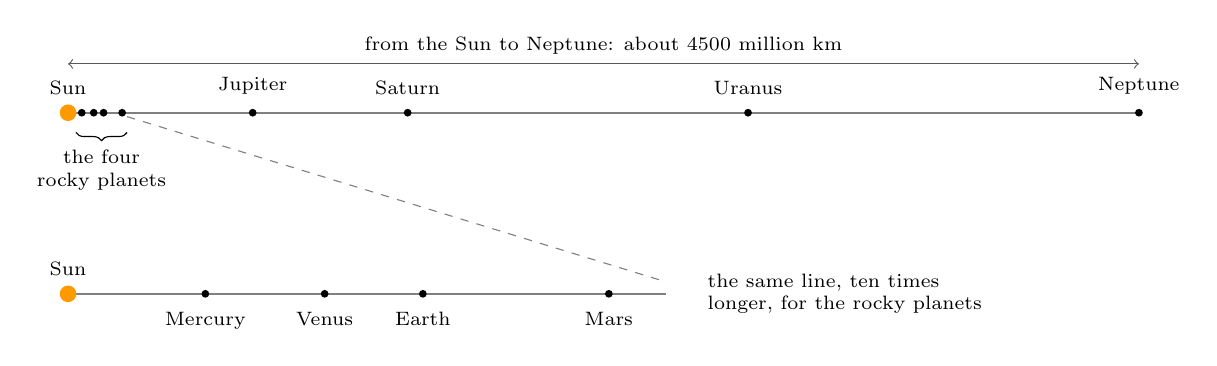
\begin{tikzpicture}
  % whole system
  \draw[thick, gray] (0,0) -- (13.6,0);
  \fill[orange!80!yellow] (0,0) circle (3pt);
  \node[font=\scriptsize, above=3pt] at (0,0) {Sun};
  \foreach \n/\x/\lab in {Mercury/0.174/, Venus/0.326/, Earth/0.451/, Mars/0.687/,
                          Jupiter/2.345/Jupiter, Saturn/4.313/Saturn, Uranus/8.636/Uranus, Neptune/13.6/Neptune} {
    \fill (\x,0) circle (1.4pt);
    \node[font=\scriptsize, above=3pt] at (\x,0) {\lab};
  }
  \draw[decorate, decoration={brace, amplitude=3pt, mirror}] (0.1,-0.25) -- (0.75,-0.25)
    node[midway, below=3pt, font=\scriptsize, align=center] {the four\\ rocky planets};
  \draw[<->, thin, gray!70!black] (0,0.62) -- (13.6,0.62) node[midway, above, font=\scriptsize, black] {from the Sun to Neptune: about 4500 million km};
  % the inner system, ten times larger
  \begin{scope}[yshift=-2.3cm]
    \draw[thick, gray] (0,0) -- (7.6,0);
    \fill[orange!80!yellow] (0,0) circle (3pt);
    \node[font=\scriptsize, above=3pt] at (0,0) {Sun};
    \foreach \n/\x in {Mercury/1.744, Venus/3.259, Earth/4.506, Mars/6.868} {
      \fill (\x,0) circle (1.4pt);
      \node[font=\scriptsize, below=3pt] at (\x,0) {\n};
    }
    \node[font=\scriptsize, anchor=west, align=left] at (8.0,0) {the same line, ten times\\ longer, for the rocky planets};
  \end{scope}
  \draw[dashed, gray] (0.75,-0.05) -- (7.6,-2.15);
\end{tikzpicture}

{\small The distances of the planets from the Sun, to scale. Top: the whole
Solar System, from the Sun to Neptune. Bottom: the four \omterm{def:g6:earth-a-planet:planet-types}{rocky planets},
enlarged ten times. The sizes of the dots are not to scale.}
% ledger: planet:Mercury.dist, planet:Venus.dist, planet:Earth.dist, planet:Mars.dist, planet:Jupiter.dist, planet:Saturn.dist, planet:Uranus.dist, planet:Neptune.dist (figdata/grade-6/planets.py, part dist)
\end{omfigure}

The four \omterm{def:g6:earth-a-planet:planet-types}{rocky planets} are all close to the Sun; the four \omterm{def:g6:earth-a-planet:planet-types}{giant planets} are
far out, with huge gaps between them. The gap between Mars and Jupiter alone, about 550~million kilometres, is more than twice the distance from the Sun to Mars.
% ledger: planet:Mars.dist, planet:Jupiter.dist

It is hard to draw sizes and distances on the same scale: the planets
become invisible dots. A \emph{\omterm{def:g2:drawing-to-map:scale}{scale} model} helps to imagine both at once.

\begin{method}[Building a scale model of the Solar System]\label{met:g6:earth-a-planet:scale-model}
\begin{enumerate}
  \item Choose the size of the Earth in the model, for example 1~cm.
  \item Find how many real kilometres 1~cm of the model stands for: divide
        the real diameter of the Earth (12\,756~km) by its size in the model.
  \item Divide every real size and every real distance by this number.
        Then change the units to something easy to picture (centimetres,
        metres, kilometres).
\end{enumerate}
% ledger: planet:Earth.diameter
\end{method}

\begin{example}[A marble for the Earth]\label{ex:g6:earth-a-planet:marble}
If the Earth is a marble 1~cm wide, 1~cm stands for 12\,756~km. The Sun,
1\,391\,400~km across, becomes a ball $1\,391\,400 \div 12\,756 \approx
109$~cm wide: a ball taller than a small child. The Earth is
150~million~km from the Sun: $149\,600\,000 \div 12\,756 \approx 11\,700$~cm,
that is about 117~metres, the length of a football pitch.
% ledger: planet:Earth.diameter, sun:R, planet:Earth.dist
\end{example}

\begin{center}\small
\begin{tabular}{|l|c|c|}
\hline
\textbf{body} & \textbf{size in the model (cm)} & \textbf{distance from the Sun (m)} \\
\hline
the Sun & 109 & --- \\
Mercury & 0.38 & 45 \\
Venus & 0.95 & 85 \\
the Earth & 1.00 & 117 \\
Mars & 0.53 & 179 \\
Jupiter & 11.21 & 610 \\
Saturn & 9.45 & 1123 \\
Uranus & 4.01 & 2248 \\
Neptune & 3.88 & 3540 \\
\hline
\end{tabular}
\end{center}
% ledger: sun:R, planet:Mercury.diameter, planet:Venus.diameter, planet:Earth.diameter, planet:Mars.diameter, planet:Jupiter.diameter, planet:Saturn.diameter, planet:Uranus.diameter, planet:Neptune.diameter, planet:Mercury.dist, planet:Venus.dist, planet:Earth.dist, planet:Mars.dist, planet:Jupiter.dist, planet:Saturn.dist, planet:Uranus.dist, planet:Neptune.dist (figdata/grade-6/planets.py, part model)

In this model, the whole Solar System as far as Neptune spreads over a
circle 7~km across, with a big ball in the middle and eight marbles and
balls, the largest the size of a grapefruit, scattered across it. The
Solar System is mostly empty space.

\section{Venus, the Earth and Mars}

Venus, the Earth and Mars are neighbours, all three \omterm{def:g6:earth-a-planet:planet-types}{rocky planets}. Venus is
almost the same size as the Earth: its diameter is 95~\% of the Earth's.
Mars is smaller: its diameter is about half of the Earth's. Yet these three
planets could hardly be more different.
% ledger: planet:Venus.diameter, planet:Earth.diameter, planet:Mars.diameter (planets.py: 94.9 %)

\paragraph{Venus.} Venus is wrapped in a thick layer of air, made mostly of
carbon dioxide, with dense \omterm{def:g4:clouds-rain-snow:cloud}{clouds} of sulfuric acid, a burning acid. Its
air is so thick that it presses on the ground 92~times as hard as the air
of the Earth presses on ours. At the surface, the temperature is about
464~$^\circ$C: hot enough to melt lead. No water can stay
liquid there.
% ledger: nasa:venus-clouds, planet:Venus.psurf, planet:Venus.Tmean

\paragraph{Mars.} Mars is a cold, dry, dusty \omterm{def:g5:weather-and-climate:desert}{desert}. Its air is also made
mostly of carbon dioxide, but it is very thin: it presses on the ground
about a hundred times less than the Earth's air. The average temperature is
$-65$~$^\circ$C. Water is found there today, but frozen: as ice in the
polar caps and under the ground near the \omterm{def:g3:continents-and-oceans:poles}{poles}. Yet Mars has not always
been like this: billions of years ago, \omterm{def:g1:landscapes-around-us:water}{rivers} flowed on Mars, \omterm{def:g1:landscapes-around-us:water}{lakes} formed
and \omterm{def:g5:water-shapes-the-land:flood}{floods} swept across it.
% ledger: nasa:mars-water, planet:Mars.psurf, planet:Mars.Tmean

\paragraph{The Earth.} Between the two, the Earth has air that presses on
the ground with about 1~bar (the unit used to compare the pressure of the
air on the planets), an average temperature of 15~$^\circ$C, and \omterm{def:g2:water-on-earth:ocean}{oceans} of
liquid water.
% ledger: planet:Earth.psurf, planet:Earth.Tmean

\begin{omfigure}
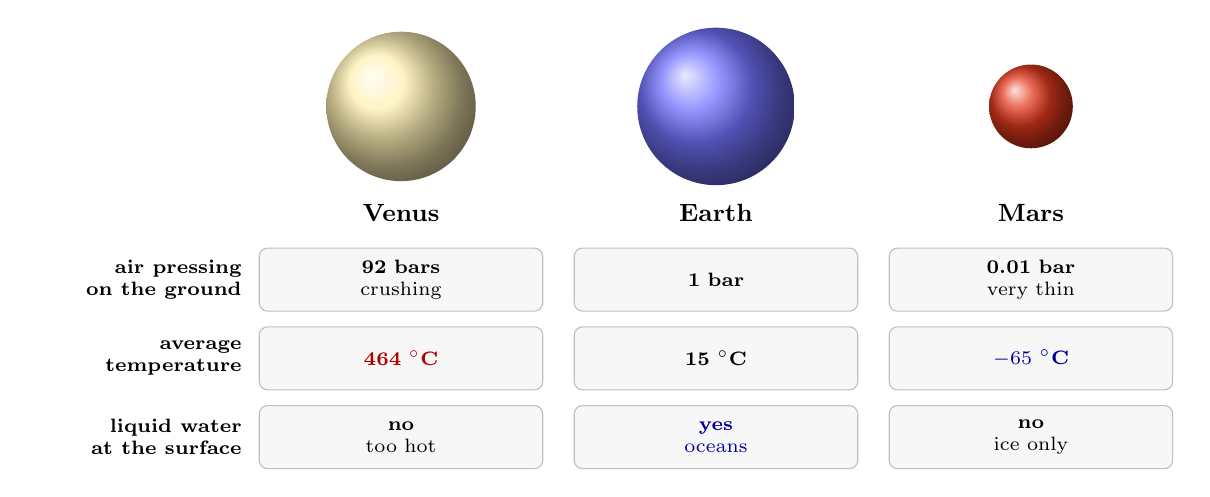
\begin{tikzpicture}[x=1cm, y=1cm,
    lab/.style={font=\scriptsize, align=center, text width=3.6cm},
    row/.style={font=\scriptsize\bfseries, anchor=east, align=right, text width=2.6cm}]
  % discs to scale: diameters 94.9 %, 100 %, 53.2 % of the Earth's (planets.py)
  \shade[ball color=yellow!60!orange!30] (3,0) circle (0.949);
  \shade[ball color=blue!55] (7,0) circle (1.0);
  \shade[ball color=red!55!brown] (11,0) circle (0.532);
  \node[font=\small\bfseries] at (3,-1.35) {Venus};
  \node[font=\small\bfseries] at (7,-1.35) {Earth};
  \node[font=\small\bfseries] at (11,-1.35) {Mars};
  \foreach \y/\t in {-2.2/{air pressing\\on the ground}, -3.2/{average\\temperature},
                     -4.2/{liquid water\\at the surface}}
    {\node[row] at (1.1,\y) {\t};}
  \foreach \x in {3,7,11}{
    \foreach \y in {-2.2,-3.2,-4.2}{
      \draw[rounded corners=3pt, black!25, fill=black!3] (\x-1.8,\y-0.4) rectangle (\x+1.8,\y+0.4);}}
  \node[lab] at (3,-2.2) {\textbf{92 bars}\\crushing};
  \node[lab] at (7,-2.2) {\textbf{1 bar}};
  \node[lab] at (11,-2.2) {\textbf{0.01 bar}\\very thin};
  \node[lab, text=red!70!black] at (3,-3.2) {\textbf{464~$^\circ$C}};
  \node[lab] at (7,-3.2) {\textbf{15~$^\circ$C}};
  \node[lab, text=blue!60!black] at (11,-3.2) {\textbf{$-65$~$^\circ$C}};
  \node[lab] at (3,-4.2) {\textbf{no}\\too hot};
  \node[lab, text=blue!60!black] at (7,-4.2) {\textbf{yes}\\oceans};
  \node[lab] at (11,-4.2) {\textbf{no}\\ice only};
\end{tikzpicture}

{\small Venus, the Earth and Mars compared. The three discs are drawn to
scale. (Values: NASA planetary fact sheet.)}
% ledger: planet:Venus.psurf, planet:Earth.psurf, planet:Mars.psurf, planet:Mercury.Tmean, planet:Venus.Tmean, planet:Earth.Tmean, planet:Mars.Tmean, planet:Jupiter.Tmean, planet:Saturn.Tmean, planet:Uranus.Tmean, planet:Neptune.Tmean, nasa:mars-water
\end{omfigure}

\paragraph{Hot and cold.} Close to the Sun, a planet receives a lot of its
light and heat; far from it, very little. So the farther a planet is from
the Sun, the colder it should be. The chart below shows that this is true
from the Earth outwards: the \omterm{def:g6:earth-a-planet:planet-types}{giant planets}, far away, are frozen worlds.
But look at Venus: it is almost twice as far from the Sun as Mercury, and
yet it is hotter! Its thick air of carbon dioxide traps the Sun's heat like
a heavy blanket and does not let it escape. Mercury, with almost no air,
cannot keep its heat.
% ledger: planet:Mercury.Tmean, planet:Venus.Tmean, planet:Earth.Tmean, planet:Mars.Tmean, planet:Jupiter.Tmean, planet:Saturn.Tmean, planet:Uranus.Tmean, planet:Neptune.Tmean, planet:Mercury.dist, planet:Venus.dist, planet:Earth.dist, planet:Mars.dist, planet:Jupiter.dist, planet:Saturn.dist, planet:Uranus.dist, planet:Neptune.dist, nasa:venus-clouds, planet:Mercury.psurf

\begin{omfigure}
\begin{tikzpicture}
  \begin{axis}[ybar, bar width=14pt, width=0.86\linewidth, height=6cm,
      ymin=-270, ymax=520, xmin=-0.6, xmax=7.6,
      xtick={0,...,7},
      xticklabels={{Mercury\\58}, {Venus\\108}, {Earth\\150}, {Mars\\228},
                   {Jupiter\\779}, {Saturn\\1432}, {Uranus\\2867}, {Neptune\\4515}},
      xticklabel style={align=center, font=\scriptsize},
      axis x line*=bottom, axis y line*=left,
      xticklabel pos=lower, ytick={-200,-100,...,500},
      ylabel={average temperature ($^\circ$C)}, xlabel={planet and distance from the Sun (million km)},
      tick label style={font=\scriptsize}, label style={font=\scriptsize},
      nodes near coords, nodes near coords style={font=\tiny},
      every node near coord/.append style={/pgf/number format/1000 sep={}}]
    \addplot[fill=orange!50, draw=black!60, bar shift=0pt]
      table[x=idx, y=tmean_C] {figdata/out/grade-6-planets-temp.dat};
    \draw[black!50] (axis cs:-0.6,0) -- (axis cs:7.6,0);
  \end{axis}
\end{tikzpicture}

{\small The average temperature of the planets, in order of distance from
the Sun. Venus breaks the rule: it is hotter than Mercury, which is closer
to the Sun. (Values: NASA planetary fact sheet.)}
% ledger: planet:Mercury.Tmean, planet:Venus.Tmean, planet:Earth.Tmean, planet:Mars.Tmean, planet:Jupiter.Tmean, planet:Saturn.Tmean, planet:Uranus.Tmean, planet:Neptune.Tmean, planet:Mercury.dist, planet:Venus.dist, planet:Earth.dist, planet:Mars.dist, planet:Jupiter.dist, planet:Saturn.dist, planet:Uranus.dist, planet:Neptune.dist (figdata/grade-6/planets.py, part temp)
\end{omfigure}

\section{What makes life possible on the Earth}

The Earth is the only planet where we know that life exists. Living things
need several conditions together, and the Earth has them all.

\begin{itemize}
  \item \textbf{Liquid water.} All living things need liquid water: the
        Earth has \omterm{def:g2:water-on-earth:ocean}{oceans}, \omterm{def:g1:landscapes-around-us:water}{rivers} and \omterm{def:g1:landscapes-around-us:water}{lakes}.
  \item \textbf{Mild temperatures.} At the Earth's surface, water freezes
        at 0~$^\circ$C and boils at 100~$^\circ$C (physics). With an
        average of 15~$^\circ$C, the Earth's temperatures stay mostly
        between the two, so its water stays liquid.
  \item \textbf{The right distance from the Sun.} Closer to the Sun, like
        Venus, a planet risks becoming too hot; farther, like Mars, too
        cold. The Earth is at the right distance for liquid water.
  \item \textbf{An atmosphere.} The layer of air around the Earth keeps its
        surface warm at night, gives living things the gases they need, and
        presses enough on the \omterm{def:g2:water-on-earth:ocean}{oceans} for their water to stay liquid. On
        Mars, the air is so thin that liquid water cannot last long at the
        surface: it freezes or turns into vapour.
\end{itemize}
% ledger: nasa:mars-water, planet:Earth.Tmean

\begin{remark}[Was there life on Mars?]\label{rem:g6:earth-a-planet:mars-life}
Since Mars once had \omterm{def:g1:landscapes-around-us:water}{rivers} and \omterm{def:g1:landscapes-around-us:water}{lakes}, scientists wonder whether tiny living
things could have lived there, long ago, when Mars was warmer and wet.
Scientists do not expect to find living things on Mars today; with robot
rovers, they look in its \omterm{def:g3:stones-pebbles-sand:rock}{rocks} for signs of life that existed long ago.
% ledger: nasa:mars-water
\end{remark}

\section{The Earth seen from space}

For thousands of years, people could only imagine what their planet looked
like from outside. On 24~December~1968, the astronauts of Apollo~8,
in orbit around the Moon, saw the Earth rise above the grey horizon of
the Moon, and one of them, Bill Anders, took the photograph below.
% ledger: nasa:earthrise

\begin{omfigure}
\begin{minipage}[c]{0.46\linewidth}\centering
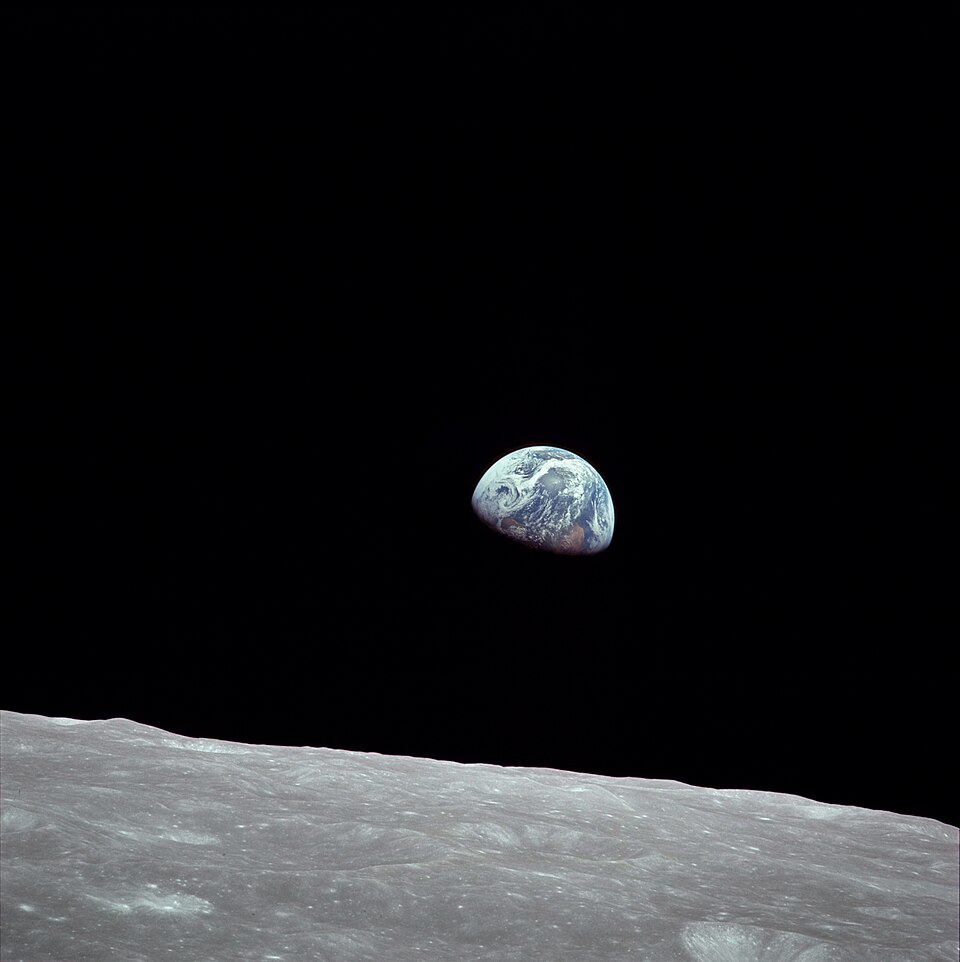
\includegraphics[width=0.85\linewidth]{images/book1/g6-earthrise.jpg}
\end{minipage}\hfill
\begin{minipage}[c]{0.5\linewidth}
{\small \emph{Earthrise}: the Earth above the horizon of the Moon,
photographed from Apollo~8 in orbit around the Moon, 24~December~1968.
(Photo: NASA, Bill Anders.)}

\medskip
{\small Look at the colours: the blue of the \omterm{def:g2:water-on-earth:ocean}{oceans}, the white swirls of
the \omterm{def:g4:clouds-rain-snow:cloud}{clouds}, the brown of the land. All around, the black of space; in the
foreground, the dead grey ground of the Moon, without water and without
air.}
\end{minipage}
% ledger: nasa:earthrise
\end{omfigure}

Seen from space, the Earth is mostly blue: the \omterm{def:g2:water-on-earth:ocean}{ocean} covers about seven
tenths of its surface. White \omterm{def:g4:clouds-rain-snow:cloud}{clouds} of water droplets swirl above it, and
white ice covers the \omterm{def:g3:continents-and-oceans:poles}{poles}. The land is brown where it is dry, green where
plants grow. The air itself cannot be seen, but the \omterm{def:g4:clouds-rain-snow:cloud}{clouds} floating in it
show that it is there. Of all the planets of the Solar System, only the Earth shows these colours
together: liquid water, \omterm{def:g4:clouds-rain-snow:cloud}{clouds} and living plants.
% ledger: wss:ocean-cover, nasa:apollo17-earth

\begin{history}[The pale blue dot]
\begin{minipage}[c]{0.66\linewidth}
On 14~February~1990, the space probe Voyager~1 was about 6~billion
kilometres from the Sun, farther out than Neptune. Before leaving the
Solar System behind, it turned its camera back and took a picture of the
Earth. In the photograph, our planet is a single bright speck, smaller than
a grain of dust, caught in a ray of sunlight. The astronomer Carl Sagan
wrote about it: ``Look again at that dot. That's here. That's home. That's
us.''
% ledger: nasa:pale-blue-dot
\end{minipage}\hfill
\begin{minipage}[c]{0.3\linewidth}\centering
\begin{tikzpicture}
  \node[inner sep=0] (img) {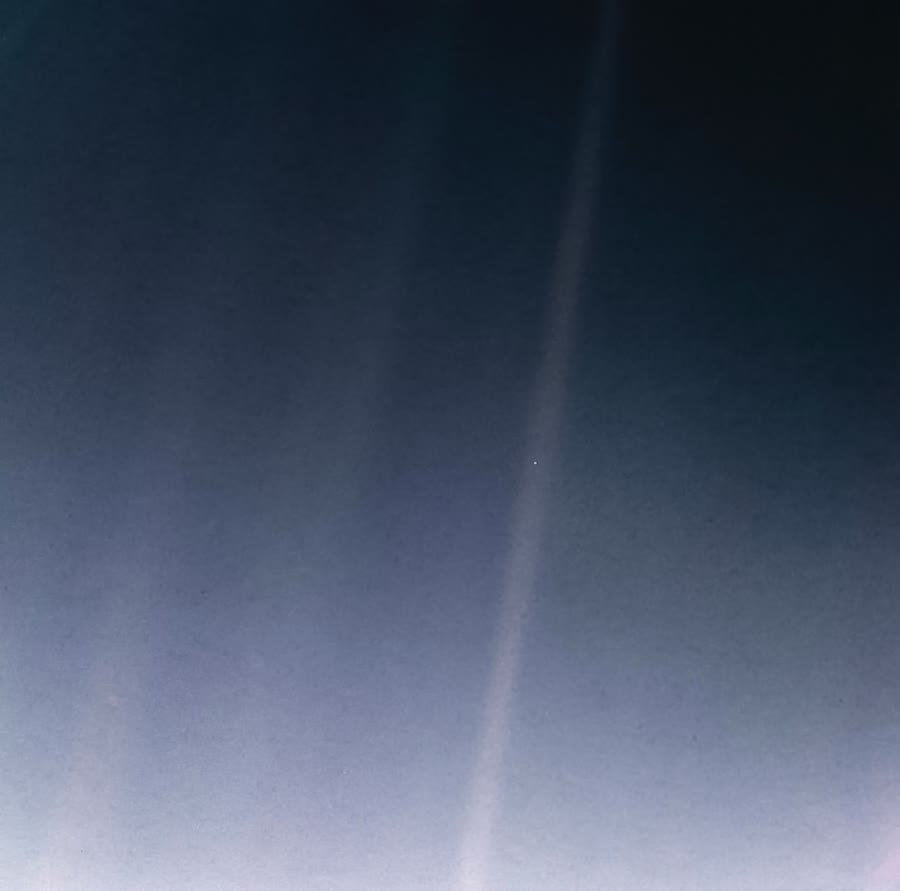
\includegraphics[width=\linewidth]{images/book1/g6-pale-blue-dot.jpg}};
  \draw[yellow!80!orange, thick] ($(img.south west)!0.594!(img.south east) + (0,{0.476*\linewidth})$) circle (6pt);
\end{tikzpicture}\\[2pt]
{\footnotesize The Earth (circled) seen by Voyager~1, 1990. (Image:
NASA/JPL-Caltech, public domain.)}
% ledger: nasa:pale-blue-dot
\end{minipage}
\end{history}

\section{Exercises}

\begin{exercise}[$\star$]\label{exo:g6:earth-a-planet:1}
List the eight planets of the Solar System in order, from the closest to
the Sun to the farthest. Underline the \omterm{def:g6:earth-a-planet:planet-types}{rocky planets}.
\end{exercise}

\begin{exercise}[$\star$]\label{exo:g6:earth-a-planet:2}
Copy and complete: ``A \omterm{def:g6:earth-a-planet:planet-types}{rocky planet} is small and \ldots, with a solid
\ldots{} A \omterm{def:g6:earth-a-planet:planet-types}{giant planet} is very large, of low \ldots, made mostly of
\ldots{} and \ldots{}''
\end{exercise}

\begin{exercise}[$\star$]\label{exo:g6:earth-a-planet:3}
Using the table of this chapter, which planet has the diameter closest to
the Earth's? Which is the largest planet? Which is the smallest?
\end{exercise}

\begin{exercise}[$\star$]\label{exo:g6:earth-a-planet:4}
True or false? Correct the false sentences.
(a) Venus is covered with \omterm{def:g2:water-on-earth:ocean}{oceans}.
(b) Mars is colder than the Earth.
(c) The \omterm{def:g6:earth-a-planet:planet-types}{giant planets} are the four planets closest to the Sun.
(d) Saturn is less dense than water.
\end{exercise}

\begin{exercise}[$\star\star$]\label{exo:g6:earth-a-planet:5}
The diameter of Mercury is 4\,879~km, the diameter of the Earth
12\,756~km. Work out the diameter of Mercury as a percentage of the
Earth's, rounded to the nearest whole number.
% ledger: planet:Mercury.diameter, planet:Earth.diameter (planets.py: 38.2 %)
\end{exercise}

\begin{exercise}[$\star\star$]\label{exo:g6:earth-a-planet:6}
How many Earths, side by side, would fit across the diameter of Saturn
(120\,536~km)? Round to the nearest whole number. Is Saturn a \omterm{def:g6:earth-a-planet:planet-types}{rocky planet}
or a \omterm{def:g6:earth-a-planet:planet-types}{giant planet}?
% ledger: planet:Saturn.diameter, planet:Earth.diameter
\end{exercise}

\begin{exercise}[$\star\star$]\label{exo:g6:earth-a-planet:7}
Astronomers have found planets around other stars. Planet~A has a density
of 1.1~grams per cubic centimetre and is 9~times as wide as the Earth.
Planet~B has a density of 5.0~grams per cubic centimetre and is a little
smaller than the Earth. Which one is a \omterm{def:g6:earth-a-planet:planet-types}{rocky planet} and which one a \omterm{def:g6:earth-a-planet:planet-types}{giant
planet}? Explain.
\end{exercise}

\begin{exercise}[$\star\star$]\label{exo:g6:earth-a-planet:8}
Using the chart of the temperatures of the planets: (a) how many degrees
hotter is Venus than the Earth? (b) How many degrees colder is Mars than
the Earth?
% ledger: planet:Venus.Tmean, planet:Earth.Tmean, planet:Mars.Tmean
\end{exercise}

\begin{exercise}[$\star\star$]\label{exo:g6:earth-a-planet:9}
Mercury is the closest planet to the Sun, but Venus is the hottest. Explain
why.
\end{exercise}

\begin{exercise}[$\star\star$]\label{exo:g6:earth-a-planet:10}
The Earth is 150~million kilometres from the Sun and Mars 228~million
kilometres. How many million kilometres farther from the Sun is Mars? By
what percentage is Mars's distance larger than the Earth's (round to the
nearest whole number)?
% ledger: planet:Earth.dist, planet:Mars.dist
\end{exercise}

\begin{exercise}[$\star\star\star$]\label{exo:g6:earth-a-planet:11}
A friend says: ``Mars has always been a dry \omterm{def:g5:weather-and-climate:desert}{desert}; there has never been
any water there.'' Using this chapter, answer him: what did Mars have
billions of years ago, where is its water today, and why can liquid water
not last at its surface now?
\end{exercise}

\begin{exercise}[$\star\star\star$]\label{exo:g6:earth-a-planet:12}
Venus is sometimes called the Earth's twin. Its diameter is 95~\% of the
Earth's, and the pull of gravity at its surface is 8.9 on a scale where the
Earth's is 9.8. (a) Work out Venus's pull of gravity as a percentage of the
Earth's,
rounded to the nearest whole number. (b) Give two ways in which Venus is
like a twin of the Earth, and two ways in which it is not.
% ledger: planet:Venus.gravity, planet:Earth.gravity, planet:Venus.diameter
\end{exercise}

\section{Problem: Postcards from three planets}

\begin{problem}[{Weekend problem --- three postcards from space, and how hard
the air of Venus presses on its ground}]
\label{pb:g6:earth-a-planet:1}
% ledger: planet:Venus.dist, planet:Venus.diameter, planet:Venus.density, planet:Venus.Tmean, planet:Venus.psurf, planet:Earth.dist, planet:Earth.diameter, planet:Earth.density, planet:Earth.Tmean, planet:Earth.psurf, planet:Mars.dist, planet:Mars.diameter, planet:Mars.density, planet:Mars.Tmean, planet:Mars.psurf, nasa:venus-clouds, nasa:mars-water
Three robot probes each send home a postcard, with a few numbers written on
the back.

\begin{center}
\small
\begin{tabular}{>{\raggedright\arraybackslash}p{0.29\linewidth}>{\raggedright\arraybackslash}p{0.29\linewidth}>{\raggedright\arraybackslash}p{0.29\linewidth}}
\hline
\textbf{From Venus} & \textbf{From the Earth} & \textbf{From Mars}\\
\hline
Distance from the Sun: 108~million~km. & Distance from the Sun:
150~million~km. & Distance from the Sun: 228~million~km.\\
Diameter: 12\,104~km. & Diameter: 12\,756~km. & Diameter: 6\,792~km.\\
Density: 5.2~g/cm$^3$. & Density: 5.5~g/cm$^3$. & Density: 3.9~g/cm$^3$.\\
Average temperature: 464~$^\circ$C. & Average temperature: 15~$^\circ$C. &
Average temperature: $-65$~$^\circ$C.\\
The air presses on the ground with 92~bars. Thick \omterm{def:g4:clouds-rain-snow:cloud}{clouds} of acid. &
The air presses on the ground with 1~bar. \omterm{def:g2:water-on-earth:ocean}{Oceans} and \omterm{def:g4:clouds-rain-snow:cloud}{clouds}. &
The air presses on the ground with 0.01~bar. Ice at the \omterm{def:g3:continents-and-oceans:poles}{poles}.\\
\hline
\end{tabular}
\end{center}

\medskip
\noindent\textbf{Part I --- The planets compared.}
\begin{enumerate}
  \item Put the three planets in order of distance from the Sun.
  \item How many million kilometres closer to the Sun than the Earth is
        Venus? How many million kilometres farther is Mars?
  \item Work out the diameter of Mars as a percentage of the Earth's,
        rounded to the nearest whole number. Is Mars about a quarter, a
        half or three quarters of the Earth's width?
  \item Are the three planets \omterm{def:g6:earth-a-planet:planet-types}{rocky planets} or \omterm{def:g6:earth-a-planet:planet-types}{giant planets}? Which numbers
        on the postcards tell you so?
\end{enumerate}

\medskip
\noindent\textbf{Part II --- The air.}
\begin{enumerate}[resume]
  \item On which planet is the air the thickest? On which is it the
        thinnest?
  \item How many times less does the air of Mars press on its ground than
        the air of the Earth on ours?
  \item Venus is closer to the Sun than the Earth, but that alone does not
        explain a temperature of 464~$^\circ$C. What does the air of Venus
        do to the Sun's heat?
  \item How many times as hard as on the Earth does the air press on the
        ground of Venus? Why must a probe that lands on Venus have very strong walls?
\end{enumerate}

\medskip
\noindent\textbf{Part III --- Water and life.}
\begin{enumerate}[resume]
  \item At the Earth's surface, water freezes at 0~$^\circ$C and boils at
        100~$^\circ$C. Using the average temperatures, explain why water is
        liquid on the Earth.
  \item What would happen to a glass of water placed on the ground of
        Venus? On the ground of Mars?
  \item Mars had \omterm{def:g1:landscapes-around-us:water}{rivers} and \omterm{def:g1:landscapes-around-us:water}{lakes} billions of years ago. What does this
        tell us about the \omterm{def:g5:weather-and-climate:climate}{climate} of Mars long ago, compared with today?
  \item Write the back of the Earth's postcard: in a few sentences, give
        four reasons why life is possible on the Earth.
\end{enumerate}
\end{problem}
